% This file was created (at least in part) by the script ParseMdtoLatex by Louis du Plessis
% (Available from https://github.com/taming-the-beast)

\documentclass[11pt]{article}
\input{preamble}

% Add your bibtex library here
\addbibresource{master-refs}


%%%%%%%%%%%%%%%%%%%%
% Do NOT edit this %
%%%%%%%%%%%%%%%%%%%%
\begin{document}
\renewcommand{\headrulewidth}{0.5pt}
\headsep = 20pt
\lhead{ }
\rhead{\textsc {BEAST v2 Tutorial}}
\thispagestyle{plain}


%%%%%%%%%%%%%%%%%%
% Tutorial title %
%%%%%%%%%%%%%%%%%%
\begin{center}

	% Enter the name of your tutorial here
	\textbf{\LARGE Tutorial using BEAST v2.7.3}\\\vspace{2mm}

	% Enter a short description of your tutorial here
	\textbf{\textcolor{mycol}{\Large MASCOT Tutorial}}\\

	\vspace{4mm}

	% Enter the names of all the authors here
	{\Large {\em Nicola F. Müller}}
\end{center}

Parameter and State inference using the approximate structured
coalescent

%%%%%%%%%%%%%%%%%
% Tutorial body %
%%%%%%%%%%%%%%%%%

\section{Background}\label{background}

Phylogeographic methods can help reveal the movement of genes between
populations of organisms. This has been widely used to quantify pathogen
movement between different host populations, the migration history of
humans, and the geographic spread of languages or the gene flow between
species using the location or state of samples alongside sequence data.
Phylogenies therefore offer insights into migration processes not
available from classic epidemiological or occurrence data alone.

The structured coalescent allows to coherently model the migration and
coalescent process, but struggles with complex datasets due to the need
to infer ancestral migration histories. Thus, approximations to the
structured coalescent, which integrate over all ancestral migration
histories, have been developed. This tutorial gives an introduction into
how a MASCOT analysis in BEAST2 can be set-up. MASCOT is short for
\textbf{M}arginal \textbf{A}pproximation of the \textbf{S}tructured
\textbf{CO}alescen\textbf{T}\citep{mueller2017mascot} and implements a structured coalescent
approximation \citep{Mueller2017}. This approximation doesn't require
migration histories to be sampled using MCMC and therefore allows to
analyse phylogenies with more than three or four states. \clearpage

\section{Programs used in this
Exercise}\label{programs-used-in-this-exercise}

\subsubsection{BEAST2 - Bayesian Evolutionary Analysis Sampling Trees
2}\label{beast2---bayesian-evolutionary-analysis-sampling-trees-2}

BEAST2 (\url{http://www.beast2.org}) is a free software package for
Bayesian evolutionary analysis of molecular sequences using MCMC and
strictly oriented toward inference using rooted, time-measured
phylogenetic trees. This tutorial is written for BEAST v2.7.x \citep{BEAST2book2014}.

\subsubsection{BEAUti2 - Bayesian Evolutionary Analysis
Utility}\label{beauti2---bayesian-evolutionary-analysis-utility}

BEAUti2 is a graphical user interface tool for generating BEAST2 XML
configuration files.

Both BEAST2 and BEAUti2 are Java programs, which means that the exact
same code runs on all platforms. For us it simply means that the
interface will be the same on all platforms. The screenshots used in
this tutorial are taken on a Mac OS X computer; however, both programs
will have the same layout and functionality on both Windows and Linux.
BEAUti2 is provided as a part of the BEAST2 package so you do not need
to install it separately.

\subsubsection{TreeAnnotator}\label{treeannotator}

TreeAnnotator is used to produce a summary tree from the posterior sample of trees using one of the available algorithms. It can also be used to summarise and visualise the posterior estimates of other tree parameters (e.g. node height).

TreeAnnotator is provided as a part of the BEAST2 package so you do not
need to install it separately.

\subsubsection{Tracer}\label{tracer}

Tracer (\url{http://tree.bio.ed.ac.uk/software/tracer}) is used to
summarise the posterior estimates of the various parameters sampled by
the Markov Chain. This program can be used for visual inspection and to
assess convergence. It helps to quickly view median estimates and 95\%
highest posterior density intervals of the parameters, and calculates
the effective sample sizes (ESS) of parameters. It can also be used to
investigate potential parameter correlations. We will be using Tracer
v1.7.2.

\subsubsection{FigTree}\label{figtree}

FigTree (\url{http://tree.bio.ed.ac.uk/software/figtree}) is a program
for viewing trees and producing publication-quality figures. It can
interpret the node-annotations created on the summary trees by
TreeAnnotator, allowing the user to display node-based statistics
(e.g.~posterior probabilities). We will be using FigTree v1.4.4. \clearpage

\section{Practical: Parameter and State inference using the approximate
structured
coalescent}\label{practical-parameter-and-state-inference-using-the-approximate-structured-coalescent}

In this tutorial we will estimate migration rates, effective population
sizes and locations of internal nodes using the marginal approximation
of the structured coalescent implemented in BEAST2, MASCOT \citep{mueller2017mascot}.

The aim is to:

\begin{itemize}

\item
  Learn how to infer structure from trees with sampling location
\item
  Get to know how to choose the set-up of such an analysis
\item
  Learn how to read the output of a MASCOT analysis
\end{itemize}

\subsection{Setting up an analysis in
BEAUti}\label{setting-up-an-analysis-in-beauti}

\subsubsection{Download MASCOT}\label{download-mascot}

First, we have to download the package MASCOT using the BEAUTi package
manager. Go to \emph{File \textgreater{}\textgreater{} Manage Packages}
and download the package MASCOT.

\begin{figure}
    \centering
    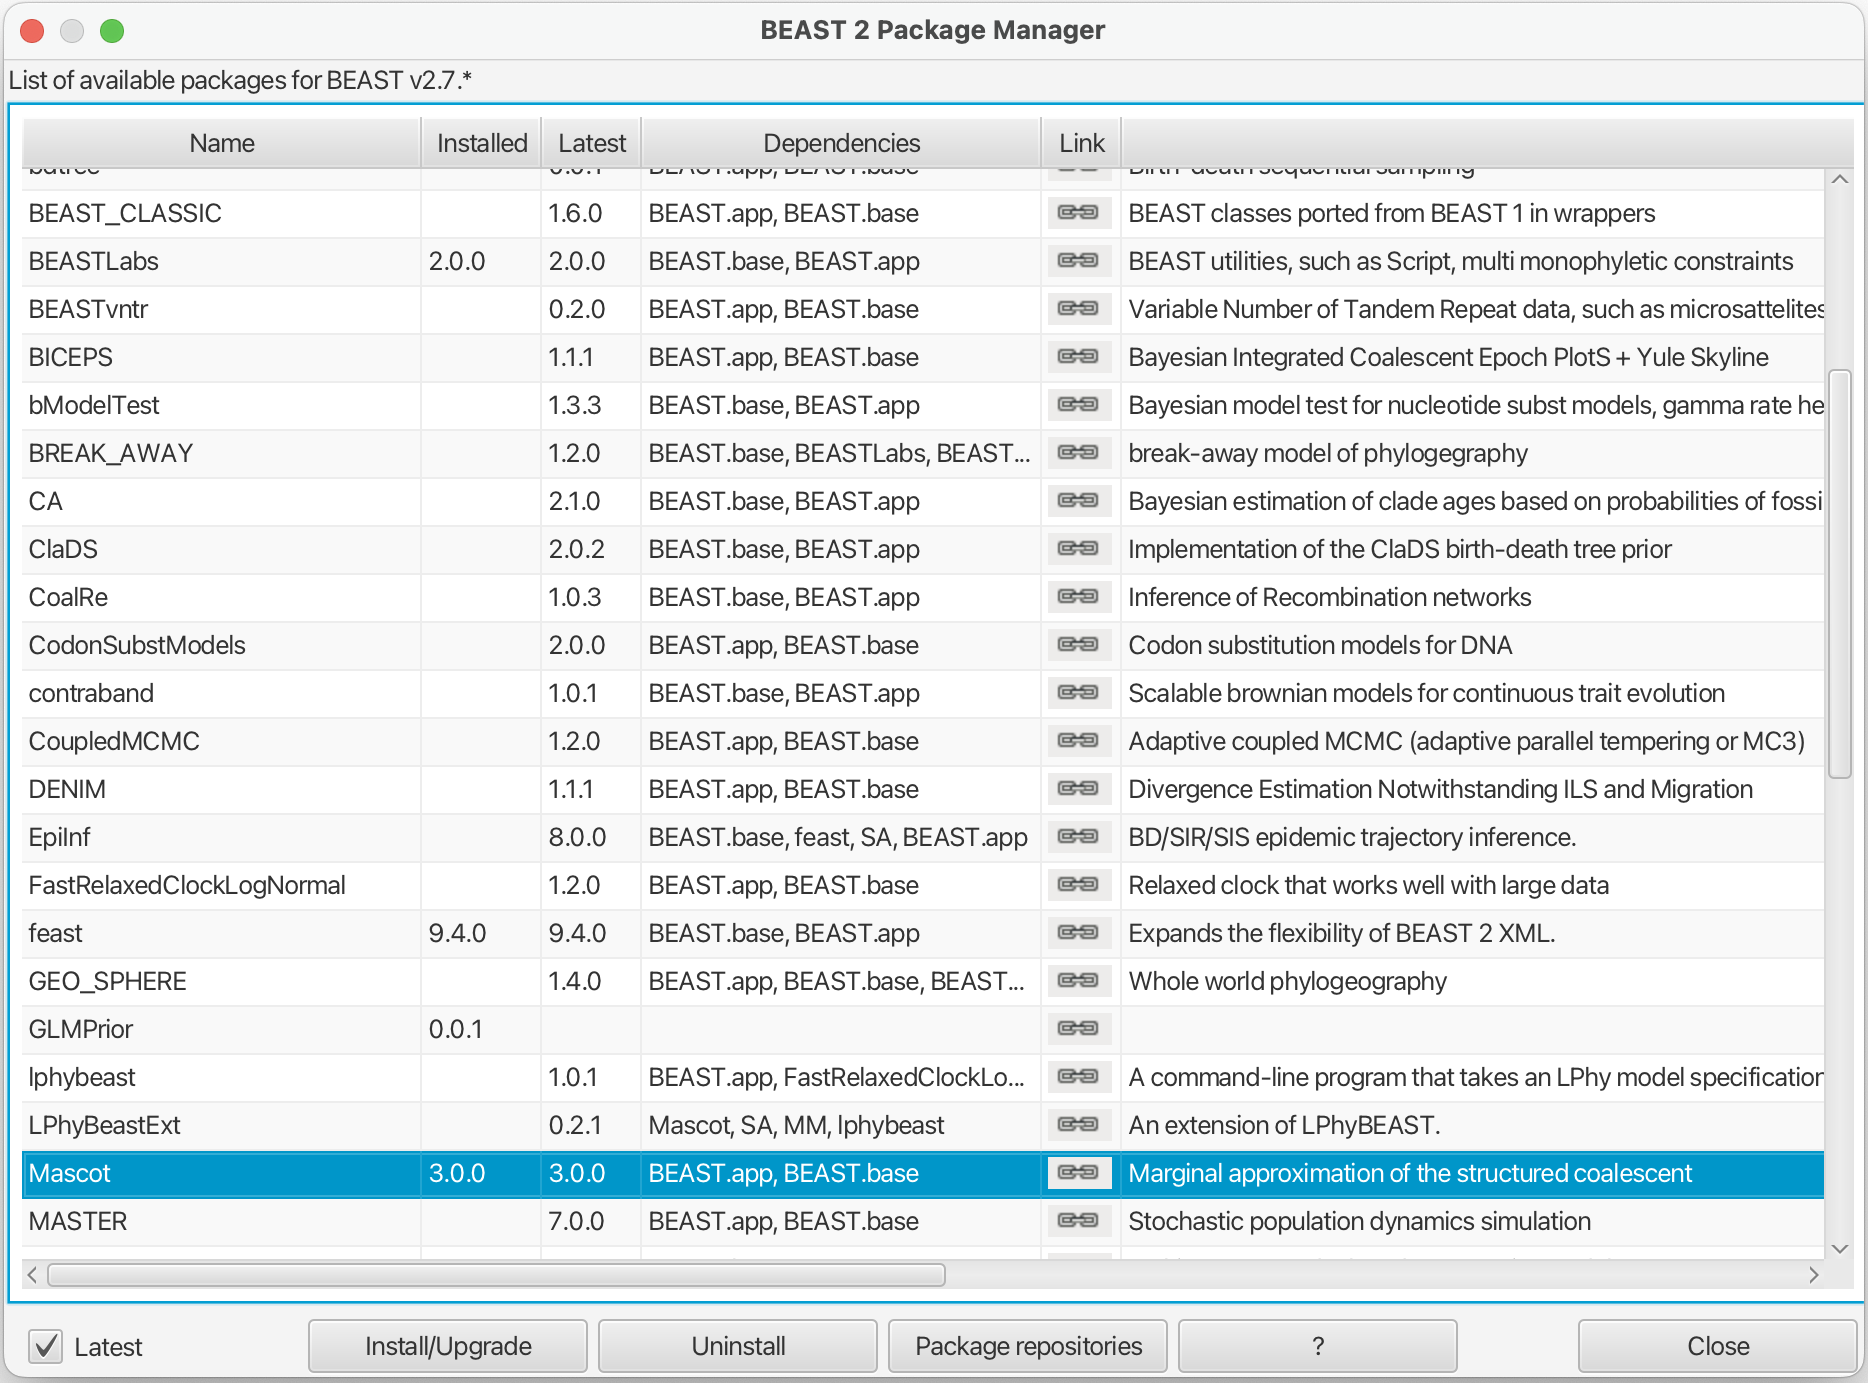
\includegraphics[width=0.500000\textwidth]{figures/MascotDownload.png}
    \caption{Download the MASCOT package.}
    \label{fig:example1}
\end{figure}

MASCOT will only be available in BEAUti once you close and restart the
program.

\subsubsection{Loading\textbf{} the Influenza A/H3N2 Sequences
(Partitions)}\label{loading-the-influenza-ah3n2-sequences-partitions}

The sequences from the \emph{data} folder name \emph{H3N2.nexus} can be
either drag and dropped into BEAUti or added using BEAUti’s menu system via \emph{File
\textgreater{}\textgreater{} Import Alignment}. Once the sequences are
added, we need to specify the sampling dates.

\subsubsection{Get the sampling times (Tip
Dates)}\label{get-the-sampling-times-tip-dates}

Open the "Tip Dates" panel and then select the "Use tip dates" checkbox.

The sampling times are encoded in the sequence names.  We can tell BEAUti 
to use these by clicking the \emph{Auto-configure} button. The sampling times 
appear following the third vertical bar "|" in the sequence name. To extract these times, select "split on character", enter "|" (without the quotes) in the text box immediately to the right, and then select "3" from the drop-down box to the right, as shown in the figure below.

\begin{figure}
    \centering
    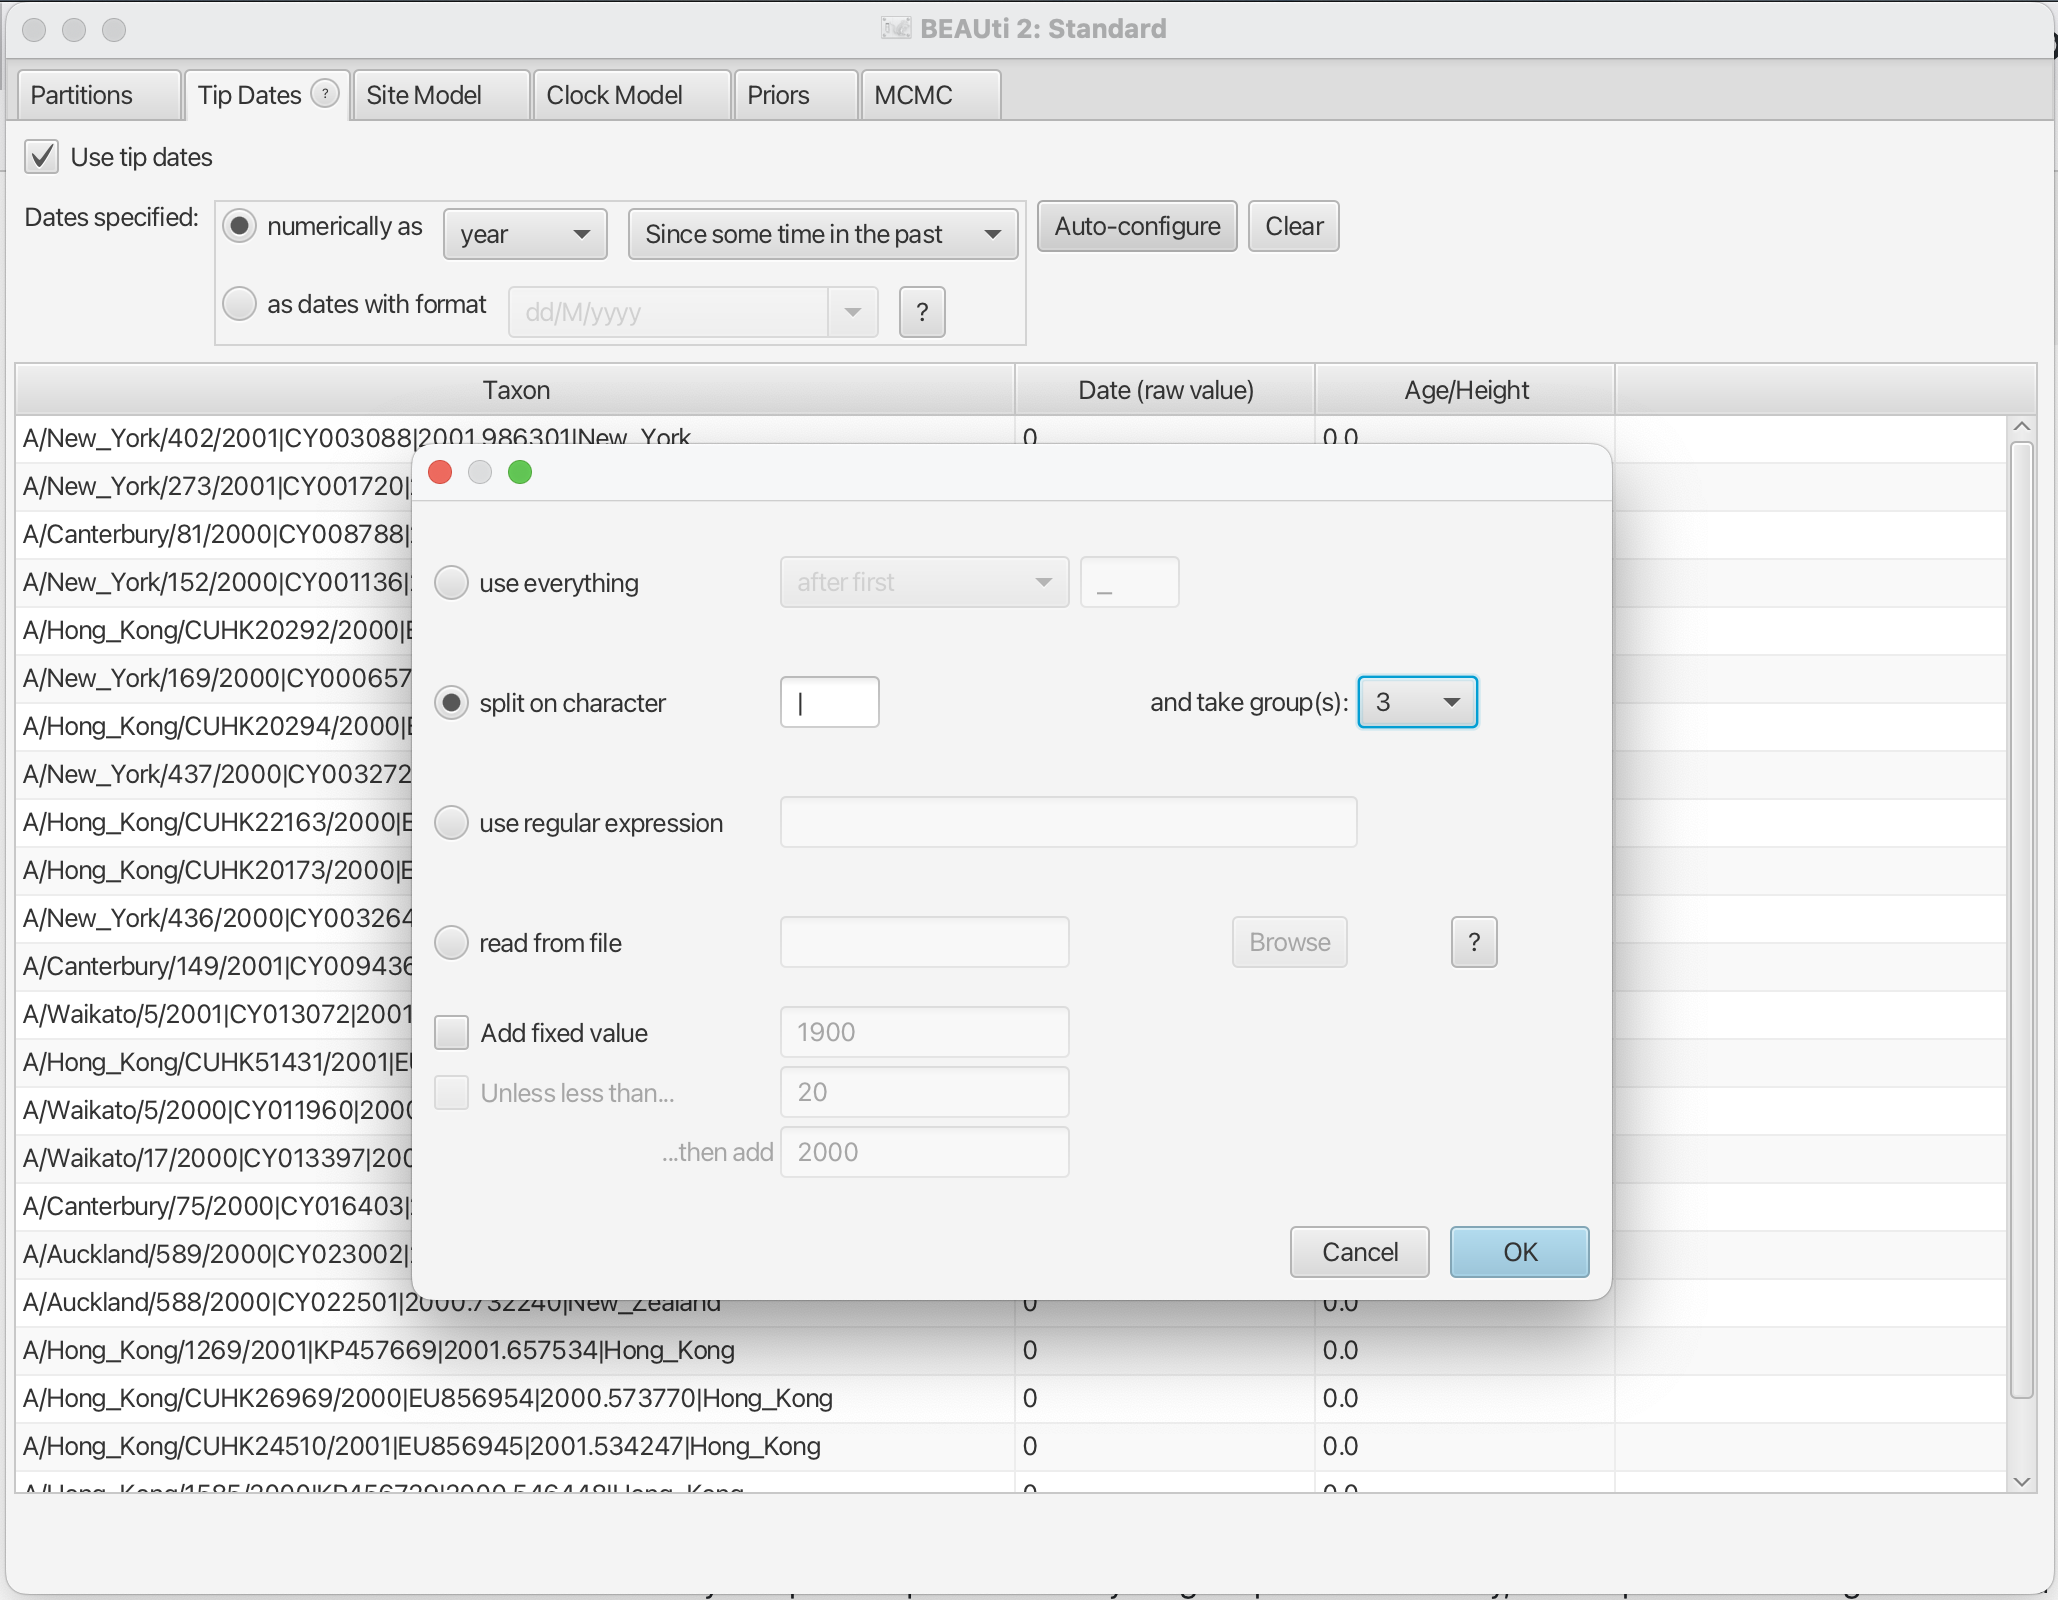
\includegraphics[width=0.700000\textwidth]{figures/TipDates.png}
    \caption{Guess sampling times.}
    \label{fig:example1}
\end{figure}

Clicking "Ok" should now populate the table with the sample times extracted from the sequence names: the column \textbf{Date} should now have values between 2000 and 2002 and the column \textbf{Height} should have values from 0 to 2. The heights denote the time difference from a sequence to the most recently sampled sequence. If everything is 
specified correctly, the sequence with Height 0.0 should have Date 2001.9. 

\subsubsection{Specify the Site Model (Site
Model)}\label{specify-the-site-model-site-model}

Next, we have to specify the site model. For Influenza Hemagluttanin
sequences as we have here, HKY is the most commonly used model of
nucleotide evolution. It allows for difference in transversion and
transition rates. Meaning that changes between bases that are chemically
closer related (transitions) are allowed to have a different rate than
changes between bases that chemically more distinct (transversion).
Additionally, we should allow for different rate categories for
different sites in the alignment. This can be done by setting the
\emph{Gamma Category Count} to 4, which is just a value that has
typically been used. Make sure that estimate is checked next to the
shape parameter. To reduce the number of parameters we have to estimate,
we can set Frequencies to Empirical.

\begin{figure}
    \centering
    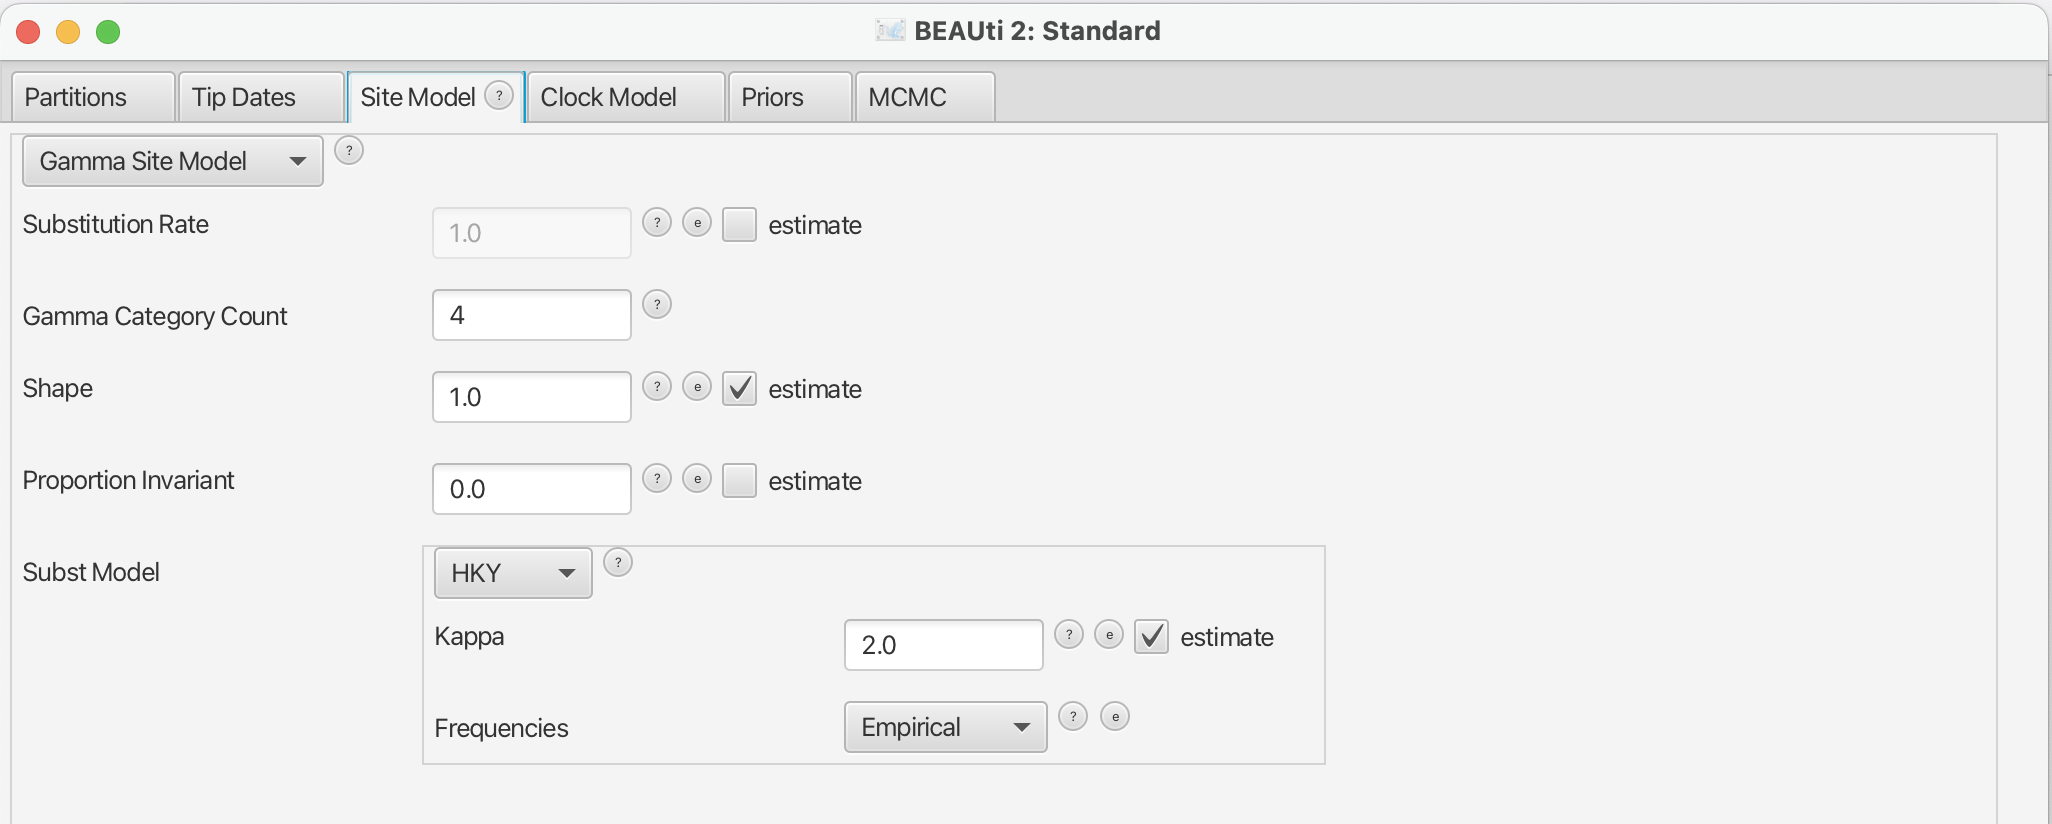
\includegraphics[width=0.700000\textwidth]{figures/SiteModel.png}
    \caption{Set the site model.}
    \label{fig:example1}
\end{figure}

\subsubsection{Set the clock model (Clock
Model)}\label{set-the-clock-model-clock-model}

For rapidly evolving viruses, the assumption of a strict molecular clock
is often made, meaning that the molecular clock is the same on each
branch of the phylogeny. To decrease the burnin phase, we can set the
initial value to 0.005.

\begin{figure}
    \centering
    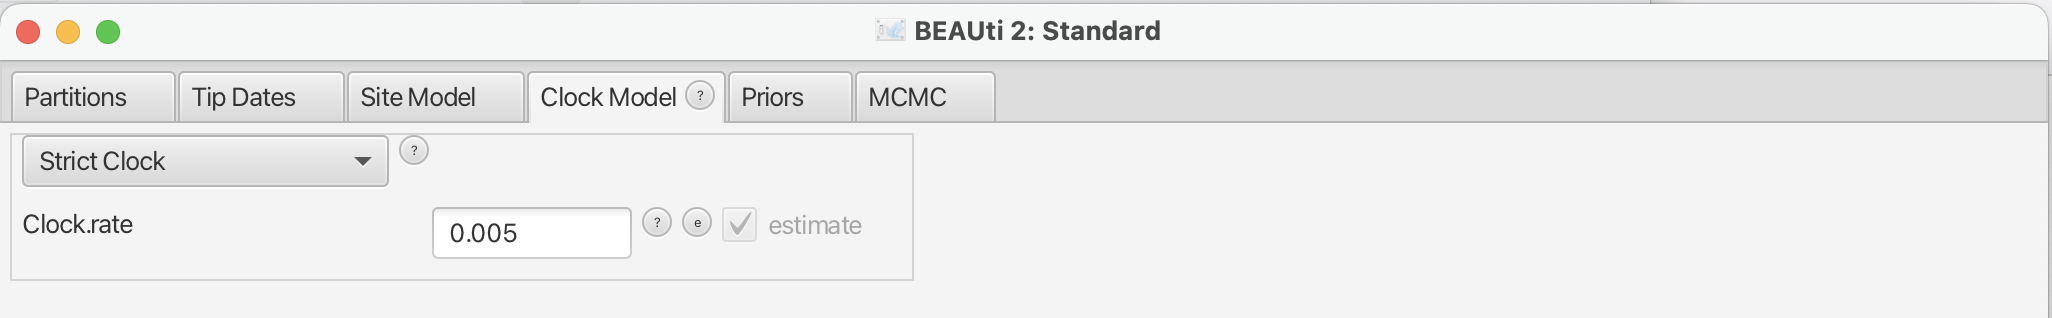
\includegraphics[width=0.700000\textwidth]{figures/ClockRate.png}
    \caption{Set the initial clock rate.}
    \label{fig:example1}
\end{figure}

\subsubsection{Get the sampling locations (Tip
Locations)}\label{get-the-sampling-times-tip-dates}

We first have to choose the tree prior, which in this case is MASCOT. 
We do this by switching to the "Priors" tab. Search the drop down menu 
next to \emph{Tree.t:H3N2} and choose MASCOT.

By default, the rate dynamics for this setting is \emph{Constant}, 
which means that effective population sizes and migration rates are assumed 
to be constant through time.
We next have to define the sampling location of the individual tips.

Initially the column \textbf{Location} should be NOT\_SET for every sequence.  
After clicking the \emph{Guess}button, you can split the sequence on the 
vertical bar "|" again by selecting "split on character" and entering "|" 
in the box. However, the locations are in the fourth group, so this time 
choose "4" from the drop-down menu.
After clicking the \emph{OK} button, the window should look like the 
one shown in the figure below:

\begin{figure}
    \centering
    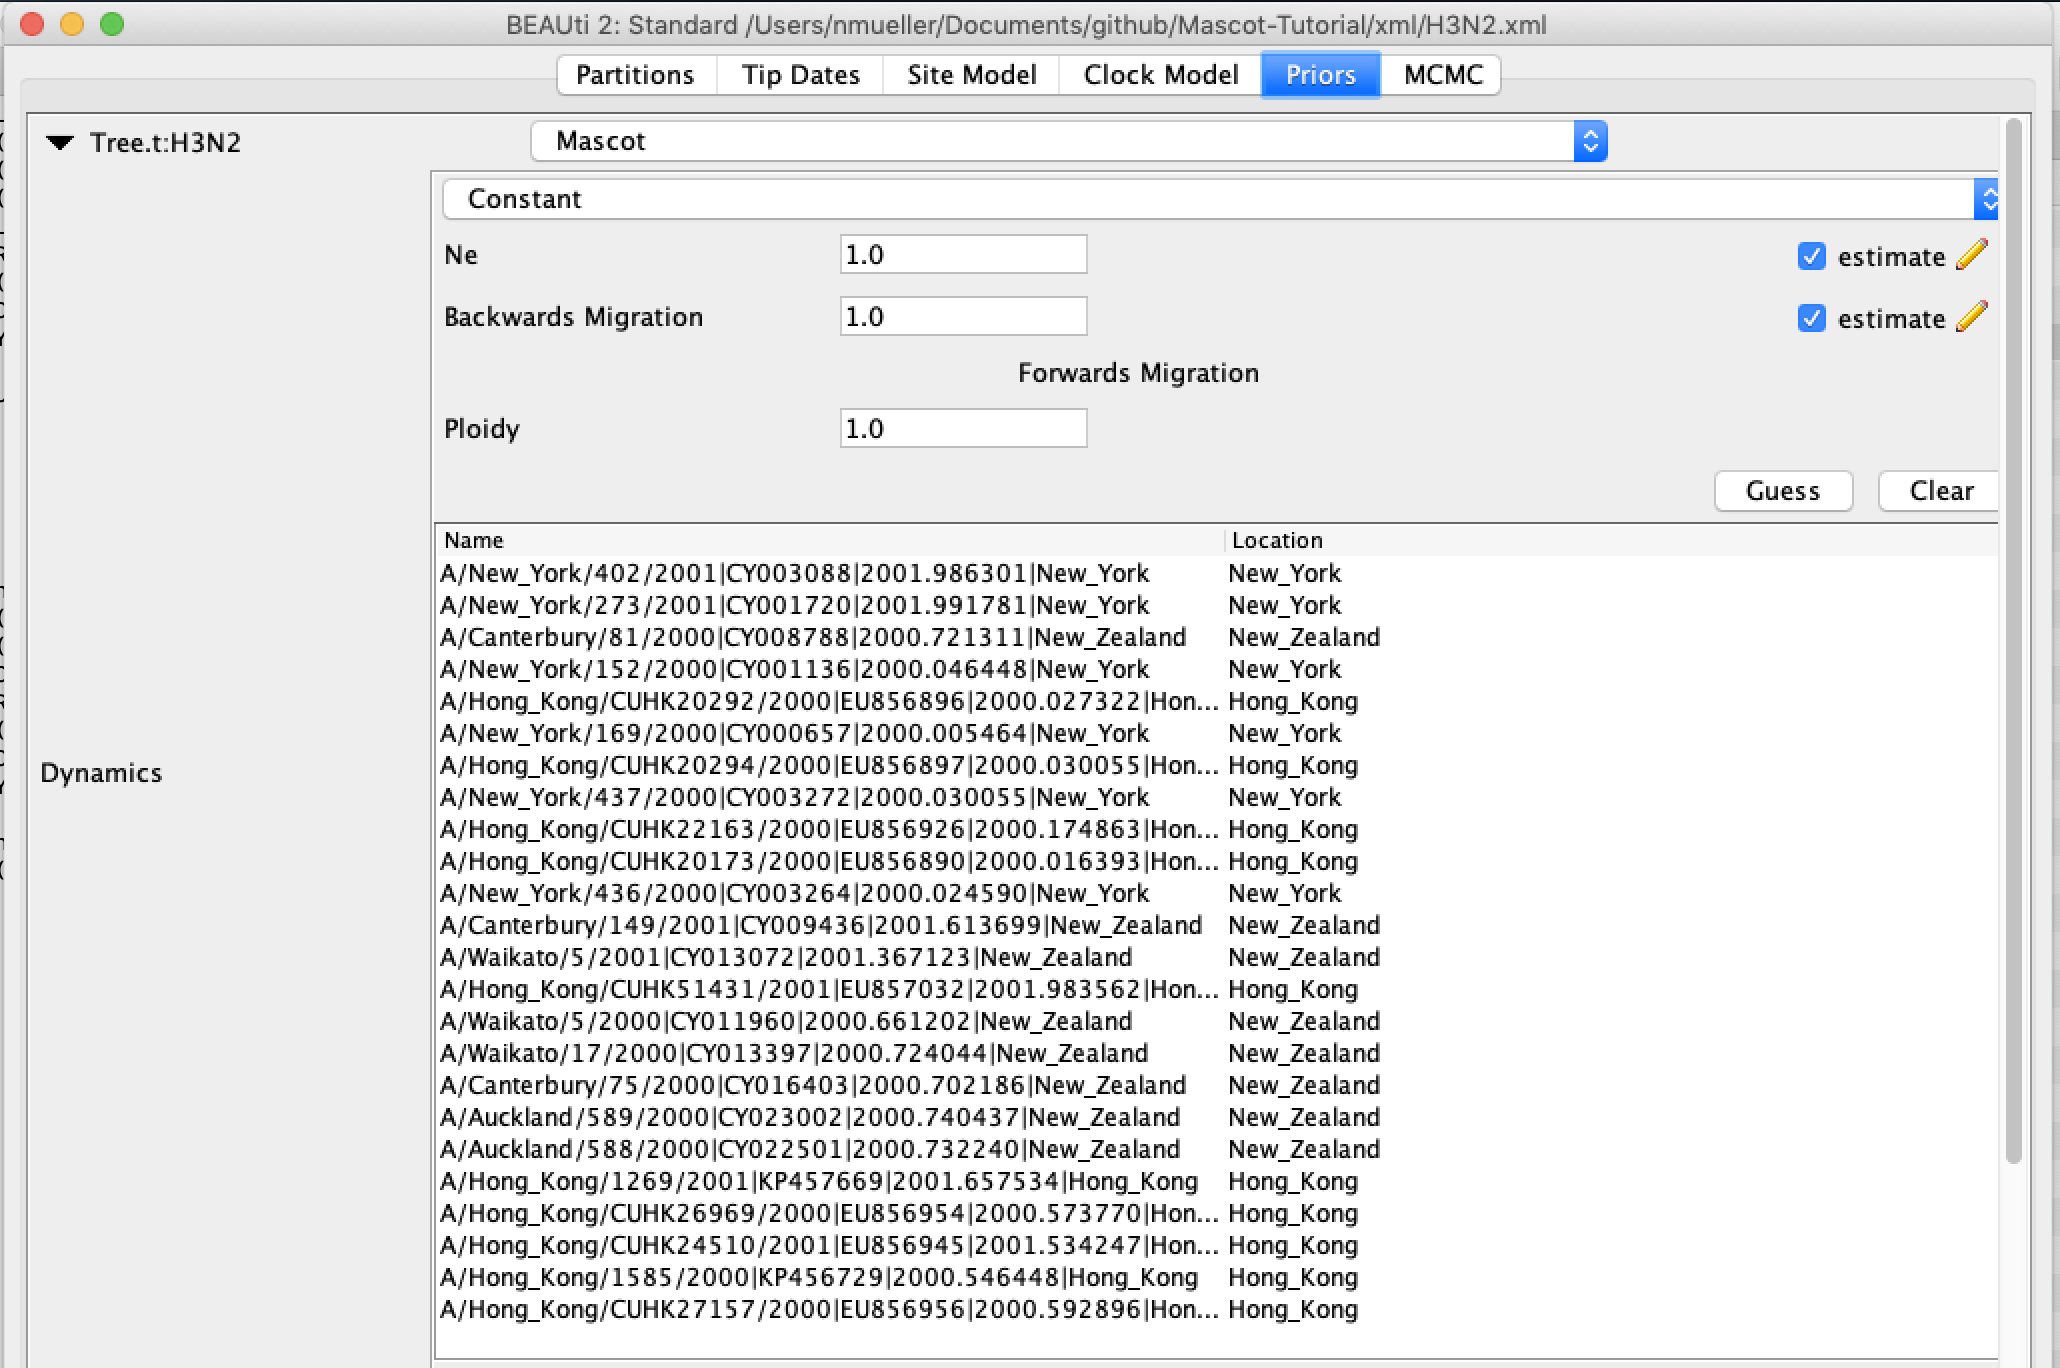
\includegraphics[width=0.700000\textwidth]{figures/TipLocations.png}
    \caption{Configuring sample locations.}
    \label{fig:example1}
\end{figure}


\subsubsection{Specify the priors (Priors)}\label{specify-the-priors-and-set-dimensions-priors}

Now, we need to set the priors for the various parameters of the model. 
You can find the parameter priors below the tree prior.

First, consider the effective population size parameter \emph{Ne}. Since we
have only a few samples per location, meaning little information about the
different effective population sizes, we will need an informative prior. 
In this case we will use a log normal prior with parameters M=0 and S=1. 
(These are respectively the mean and variance of the corresponding normal 
distribution in log space.) To use this prior, choose "Log Normal" from 
the drop down menu to the right of the \emph{Ne.t:H3N2} parameter label, 
then click the arrow to the left of the same label and fill in the parameter 
values appropriately (i.e. M=0 and S=1). Ensure that the "Mean In Real Space" 
checkbox remains unchecked.

The existing exponential distribution as a prior on the migration rate puts 
much weight on lower values while not prohibiting larger ones. For migration 
rates, a prior that prohibits too large values while not greatly distinguishing between very small and very \textbf{very} small values is generally a good choice. 
Be aware however that the exponential distribution is quite an informative prior: one should be careful that to choose a mean so that feasible rates are at least within the 95\% HPD interval of the prior.  (This can be determined by clicking the arrow to the left of the parameter name and looking at the values below the graph that appears on the right.) We keep the default mean value of 1.

Finally, set the prior for the clock rate. We have a good idea about the clock 
rate of Influenza A/H3N2 Hemagglutinin. From previous work by other people, 
we know that the clock rate will be around 0.005 substitution per site per year. To include that prior knowledge, we can set the prior on the clock rate to a Log Normal distribution with mean in \textbf{real space} set to 0.005. To specify the mean in real space, make sure that the box "Mean In Real Space" is checked. If  we set the S value to 0.25, we say that we expect the clock rate to be with 95\%  certainty between 0.00321 and 0.00731.

\begin{figure}
    \centering
    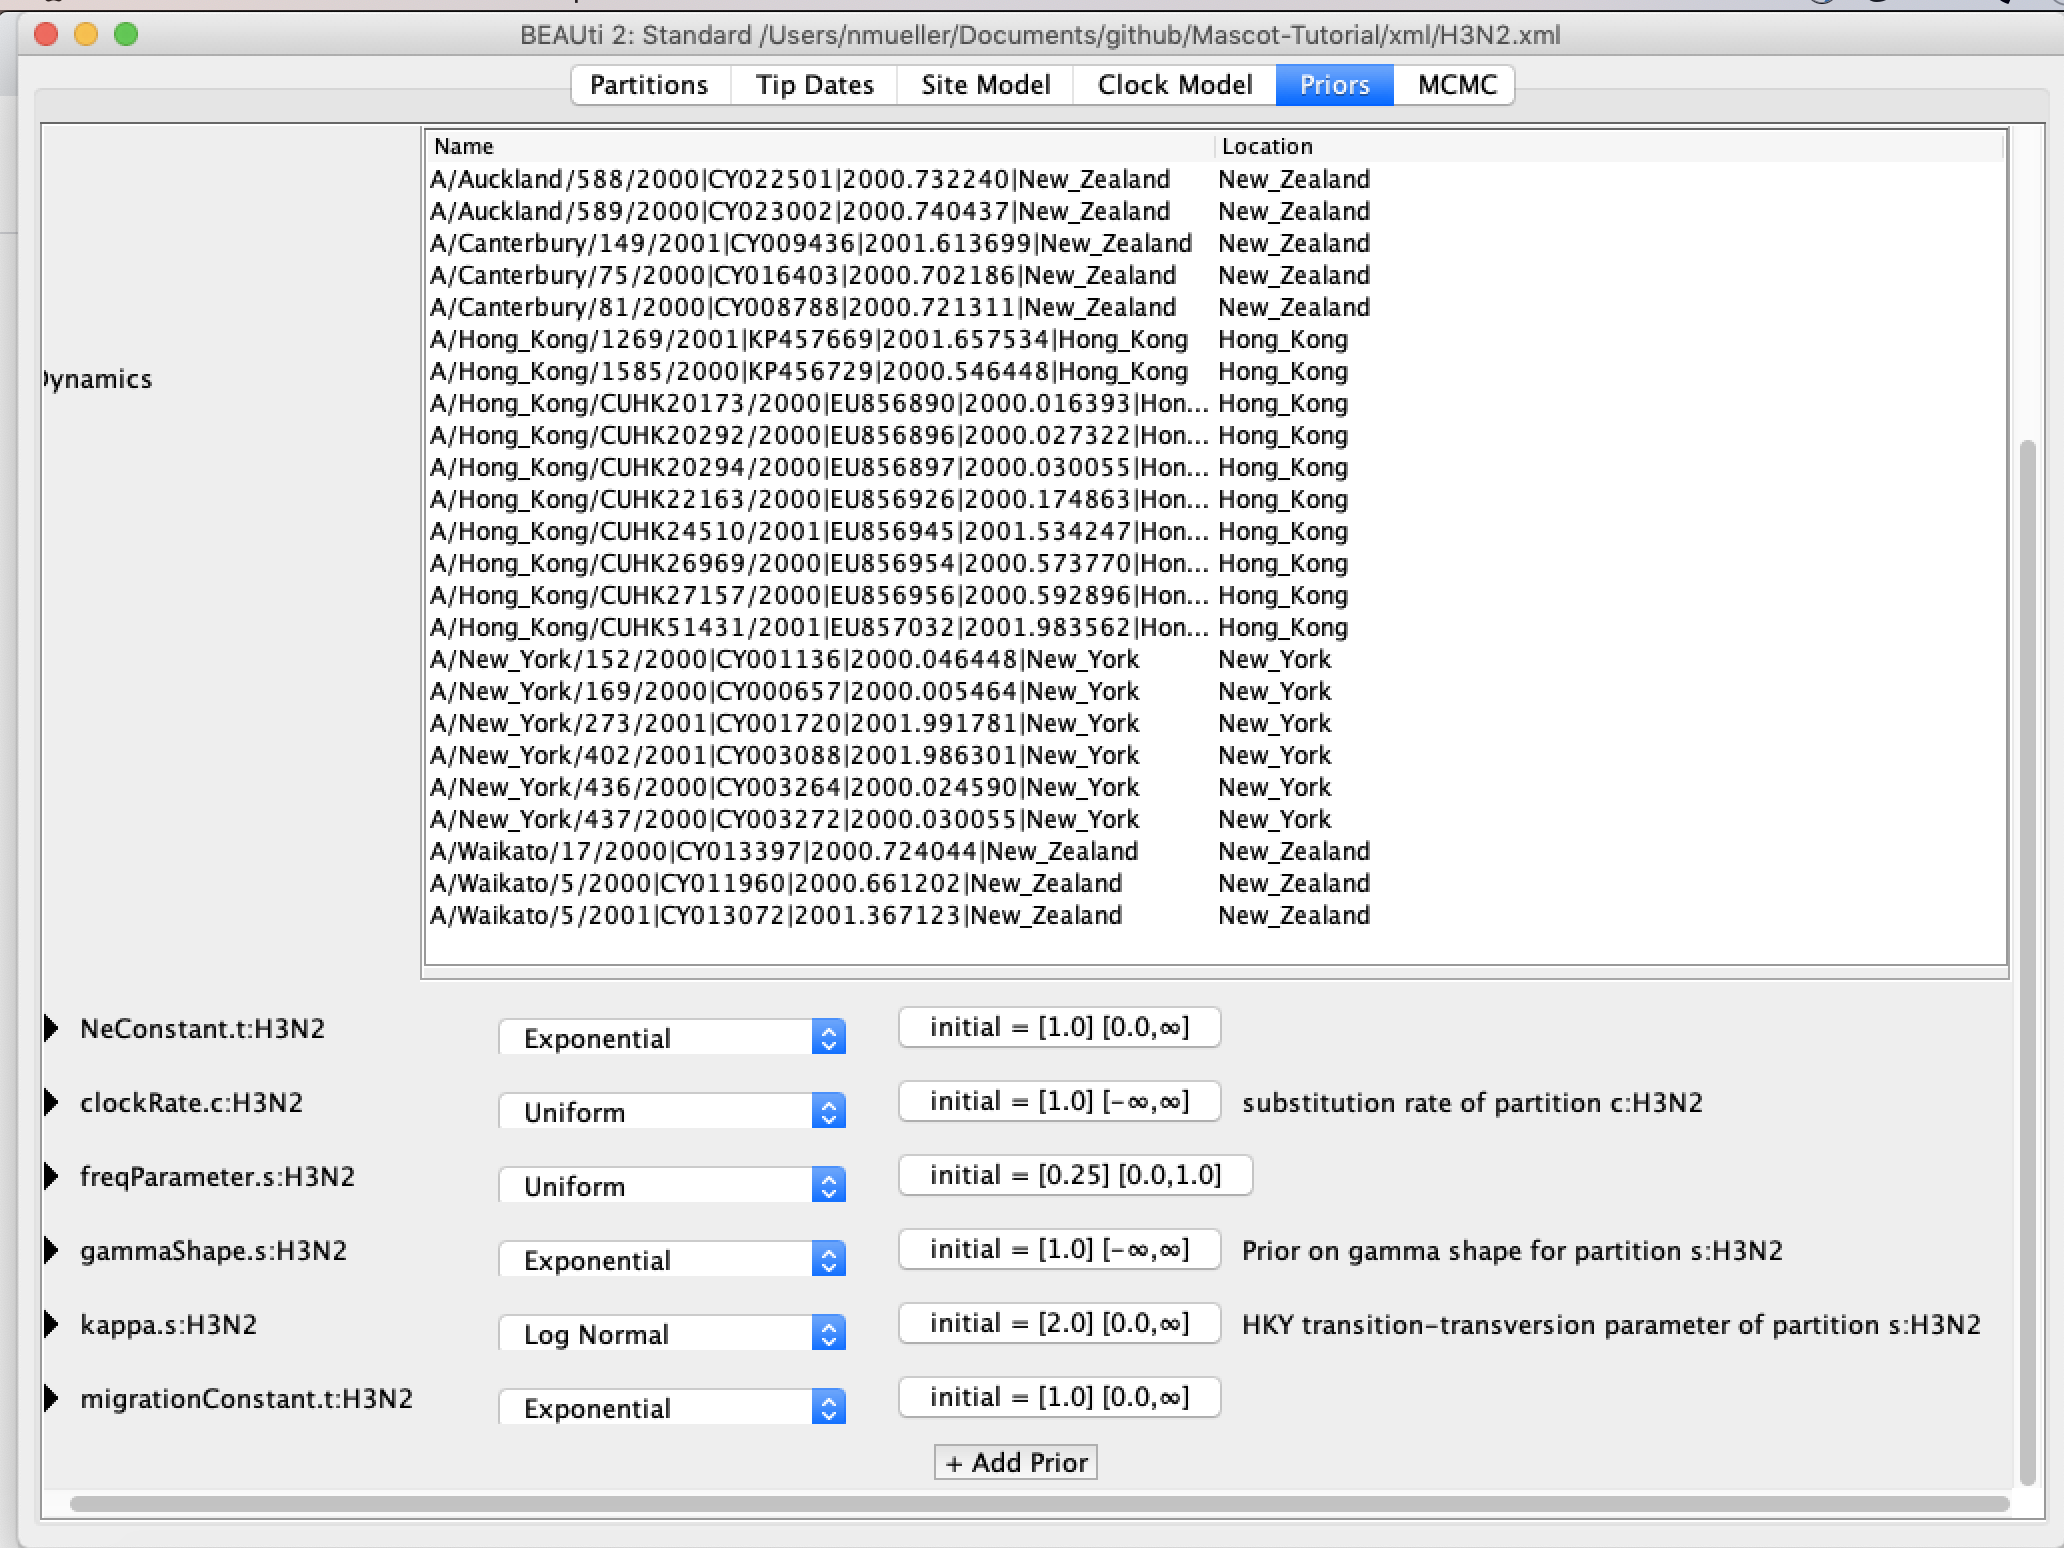
\includegraphics[width=0.700000\textwidth]{figures/Priors.png}
    \caption{Set up of the prior distributions.}
    \label{fig:example1}
\end{figure}

We keep the default priors for the parameters gammaShape and kappa.


\subsubsection{Specify the MCMC chain length
(MCMC)}\label{specify-the-mcmc-chain-length-mcmc}

Here we can set the length of the MCMC chain and after how many
iterations the parameter and trees a logged. For this dataset, 2 million
iterations should be sufficient. In order to have enough samples but not
create too large files, we can set the logEvery to 2000, so we have 1001
samples overall. Next, we have to save the \lstinline!*.xml! file under
\emph{File \textgreater{}\textgreater{} Save as}.

\begin{figure}
    \centering
    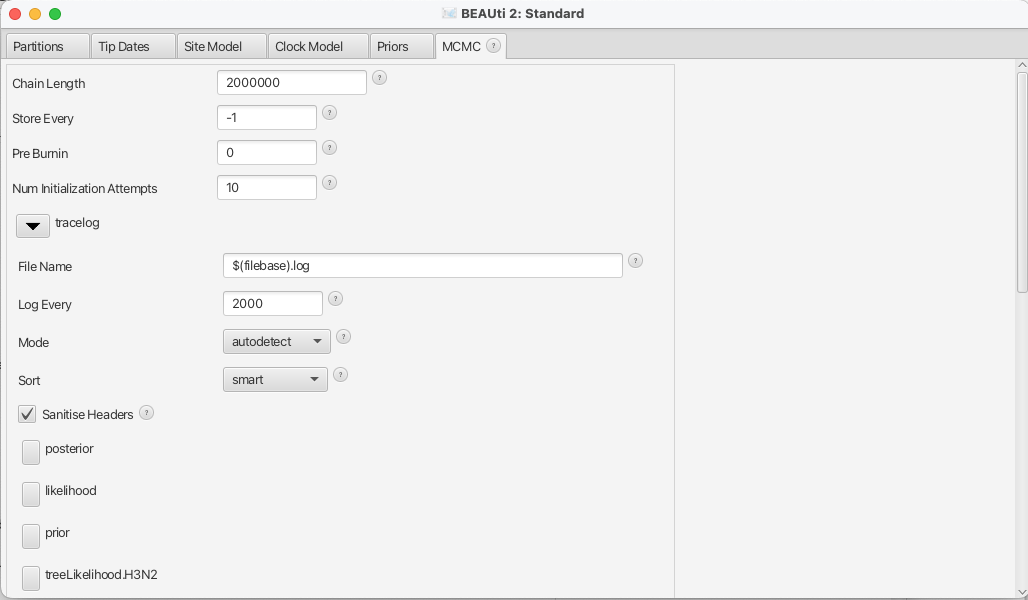
\includegraphics[width=0.700000\textwidth]{figures/MCMC.png}
    \caption{save the *.xml.}
    \label{fig:example1}
\end{figure}

\subsubsection{Run the Analysis using
BEAST2}\label{run-the-analysis-using-beast2}

Run the \lstinline!*.xml! using BEAST2 or use finished runs from the
\emph{precooked-runs} folder. The analysis should take about 6 to 7
minutes.

\subsubsection{Analyse the log file using
Tracer}\label{analyse-the-log-file-using-tracer}

First, we can open the \lstinline!*.log! file in tracer to check if the
MCMC has converged. The ESS value should be above 200 for almost all
values and especially for the posterior estimates. 

\begin{figure}
    \centering
    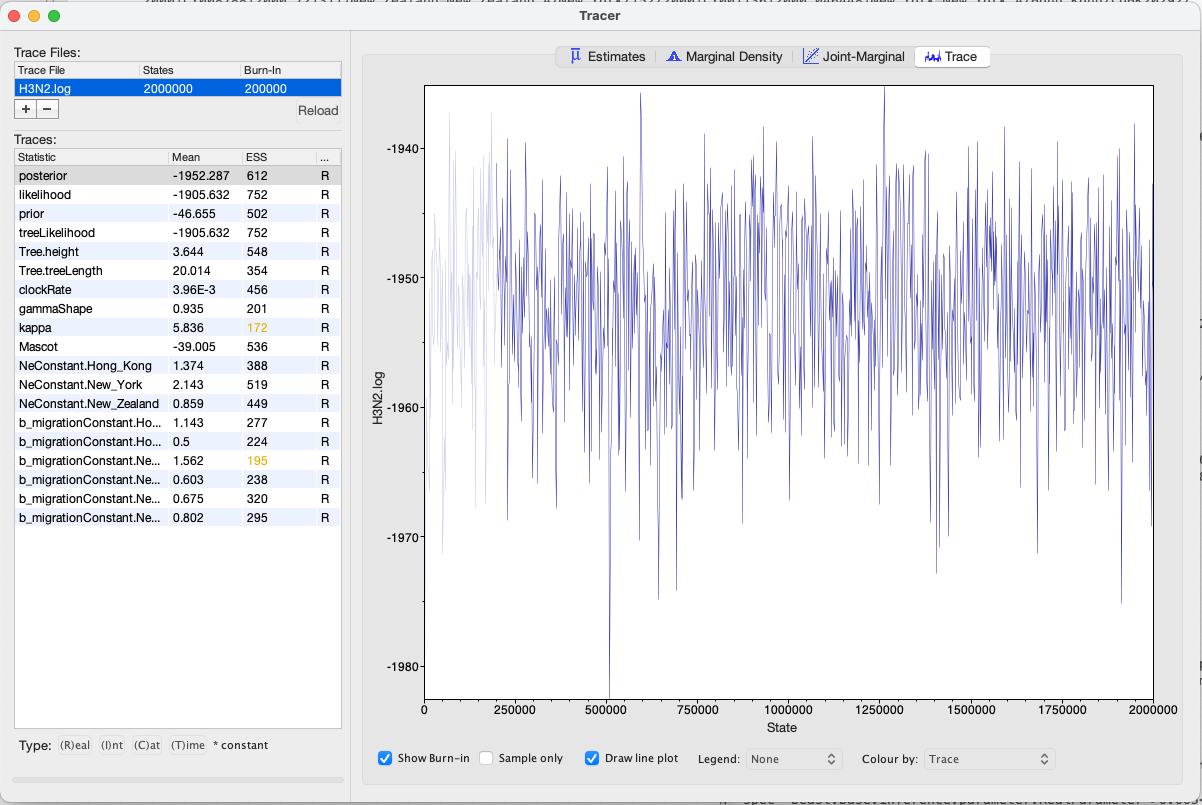
\includegraphics[width=0.700000\textwidth]{figures/LogPosterior.png}
    \caption{Check if the posterior converged.}
    \label{fig:example1}
\end{figure}

Next, we can have a look at the inferred effective population sizes. New
York is inferred to have the largest effective population size before
Hong Kong and New Zealand. This tells us that two lineages that are in
the New Zealand are expected to coalesce quicker than two lineages in
Hong Kong or New York.

\begin{figure}
    \centering
    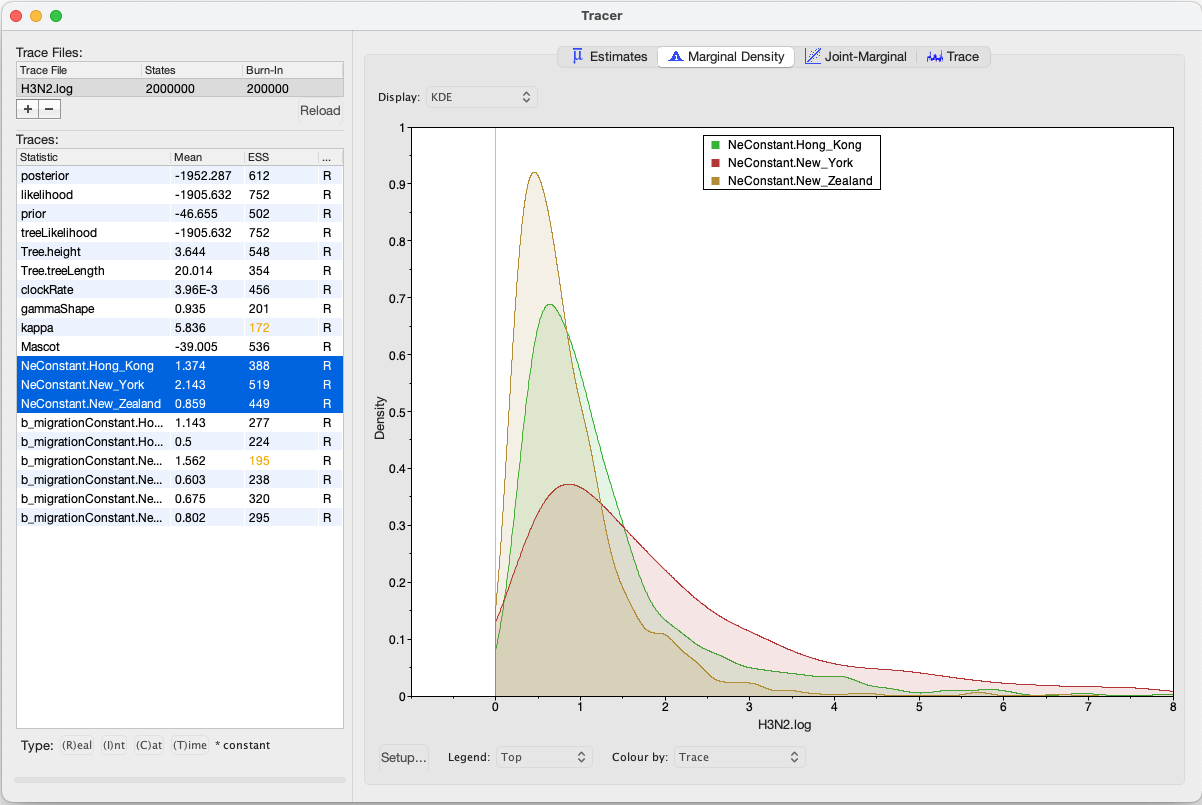
\includegraphics[width=0.700000\textwidth]{figures/LogNe.png}
    \caption{Compare the different inferred effective population sizes.}
    \label{fig:example1}
\end{figure}

In this example, we have relatively little information about the
effective population sizes of each location. This can lead to estimates
that are greatly informed by the prior. Additionally, there can be great
differences between median and mean estimates. The median estimates are
generally more reliable since they are less influence by extreme values.

\begin{figure}
    \centering
    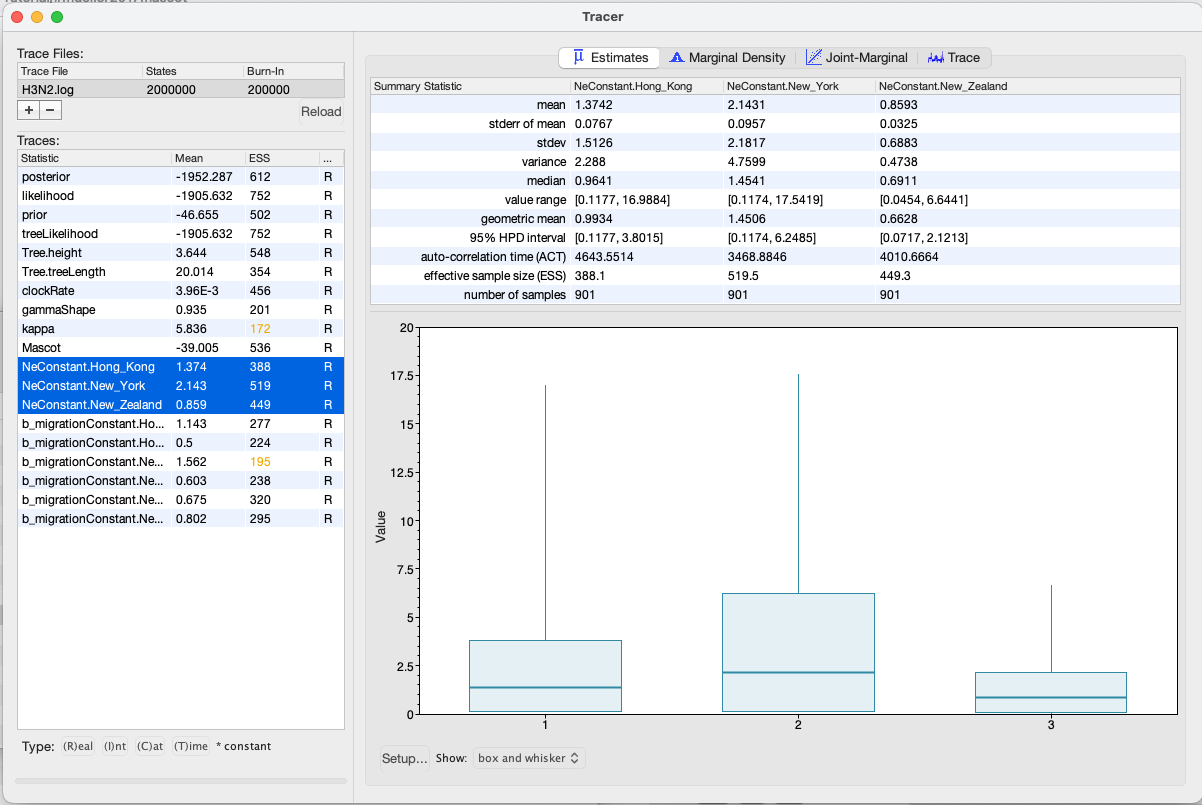
\includegraphics[width=0.700000\textwidth]{figures/MeanMedian.png}
    \caption{Differences between Mean and Meadian estimates.}
    \label{fig:example1}
\end{figure}

We can then look at the inferred migration rates. The migration rates
have the label b\_migration.*, meaning that they are backwards in time
migration rates. The highest rates are from New York to Hong Kong.
Because they are backwards in time migration rates, this means that
lineages from New York are inferred to be likely from Hong Kong if we're
going backwards in time. In the inferred phylogenies, we should
therefore make the observation that lineages ancestral to samples from
New York are inferred to be from the Hong Kong backwards.

\begin{figure}
    \centering
    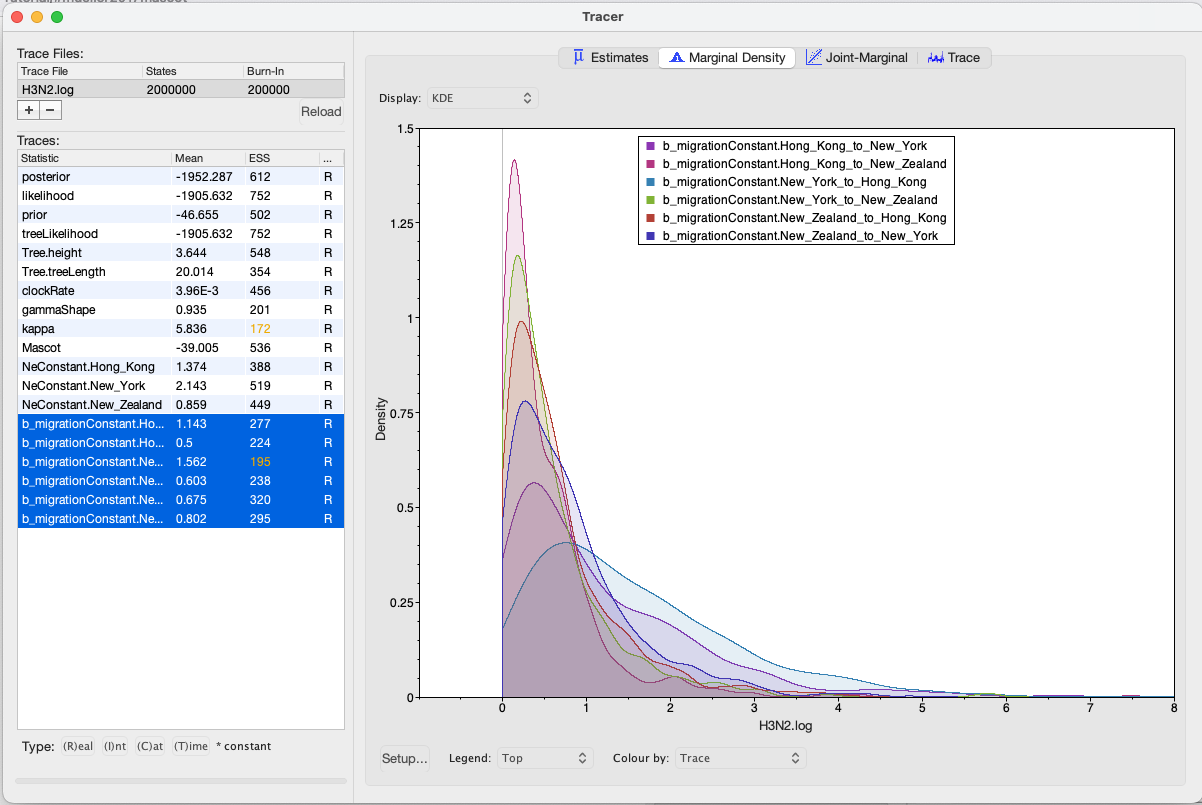
\includegraphics[width=0.700000\textwidth]{figures/LogMigration.png}
    \caption{Compare the inferrred migration rates.}
    \label{fig:example1}
\end{figure}

\subsubsection{Make the summary tree using TreeAnnotator}\label{make-the-summary-tree}

Next, we want to summarize the trees. This we can do using TreeAnnotator. Until recently the \textit{maximum clade credibility} tree (MCC) has been the default summary method in TreeAnotator. To produce MCC trees TreeAnotator takes the set of trees and find the best supported tree by maximising the product of the posterior clade probabilities. It will then annotate this representative summary tree with the mean ages of all the nodes and the corresponding 95\% HPD ranges as well as the posterior clade probability for each node. A new point estimate, called a \textit{conditional clade distribution} tree (CCD) has been proposed  \citep{berling2025}. It has been shown to outperform MCC in terms of accuracy (based on Robinson-Foulds distance to the true tree) and precision (how different are the point estimates calculated for replicate MCMC chains). CCD methods may produce a tree that would be well supported but has not been sampled during MCMC. This is beneficial for large trees and complex parameter regimes. Since both methods are still widely used, we show how to use them to summarise the posterior tree distribution. \textbf{To save time, you may run just one method and compare it to the other using the example below.}


\textbf{Producing MCC tree}

\begin{framed}
Open \textbf{TreeAnnotator} and then set the options as in the Figure \ref{fig:example1} below. You have to specify the \textbf{Burnin percentage}, \textbf{Target tree type},  \textbf{Node heights}, \textbf{Input Tree File} and the \textbf{Output File}.
Use the typed trees in the file  \lstinline!H3N2.H3N2.trees! as \textbf{Input Tree File}. Name output file \lstinline!H3N2.mcc.tree!.
After clicking \textbf{Run} the program should summarize the trees.
\end{framed}

\begin{figure}
    \centering
    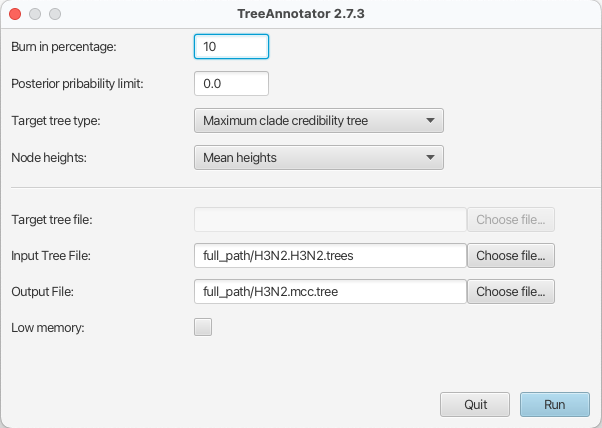
\includegraphics[width=0.500000\textwidth]{figures/TreeAnnotator.png}
    \caption{Make the maximum clade credibility tree.}
    \label{fig:example1}
\end{figure}

\textbf{Producing CCD0 tree}

To produce CCD0 summary tree, you will first need to install the CCD package.

\begin{framed}
	Open BEAUTi and select \textbf{File} >> \textbf{Manage packages}
	
	Select \textbf{CCD} package in the list and select \textbf{Install/Upgrade} (see Figure \ref{fig:installCCD})
	
	Close BEAUTi
\end{framed}

\begin{figure}[h]
	\centering
	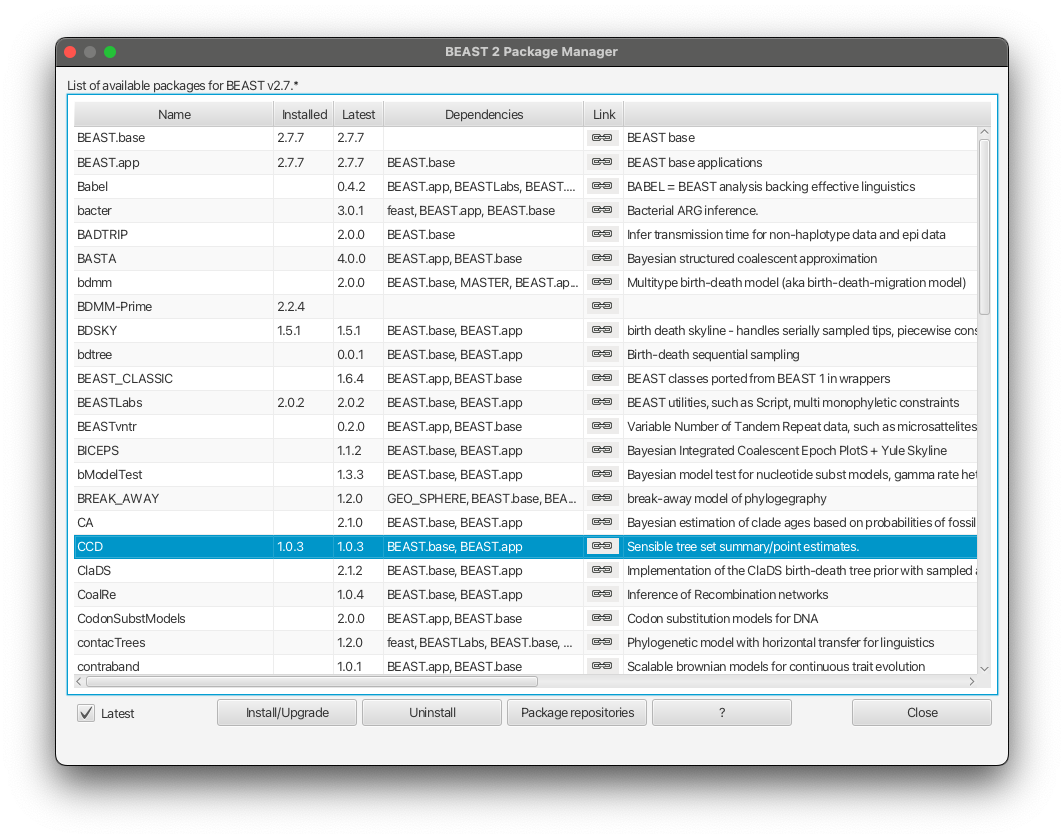
\includegraphics[width=0.600000\textwidth]{figures/installCCD0.png}
	\caption{Install CCD package.}
	\label{fig:installCCD}
\end{figure}

Now you can proceed to make CCD0 tree:

\begin{framed}
	Open \textbf{TreeAnnotator} and then set the options as in the Figure \ref{fig:ccd0} below. You have to specify the \textbf{Burnin percentage}, \textbf{Target tree type}, \textbf{Node heights}, \textbf{Input Tree File} and the \textbf{Output File}.
	Use the typed trees in the file  \lstinline!H3N2.H3N2.trees! as \textbf{Input Tree File}. Name output file \lstinline!H3N2.ccd0.tree!.
	After clicking \textbf{Run} the program should summarize the trees.
\end{framed}

\begin{figure}
	\centering
	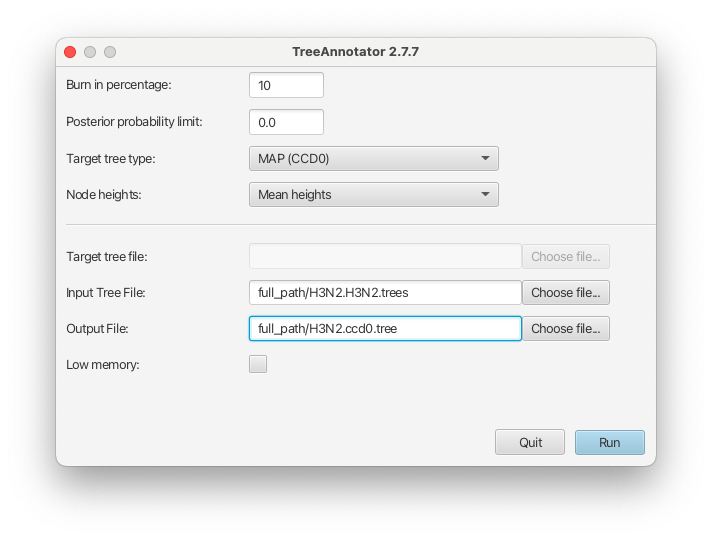
\includegraphics[width=0.600000\textwidth]{figures/treeannotator.ccd0.png}
	\caption{Make the conditional clade credibility tree.}
	\label{fig:ccd0}
\end{figure}

\subsubsection{Analyse and compare the MCC and CCD0 summary trees}\label{analyse-and-compare-summary-tree}

In each logging step of the tree during the MCMC, MASCOT logs several different things. It logs the inferred probability of each node being in any possible location. In this example, these would be the inferred probabilities of being in Hong Kong, New York and New Zealand. Additionally, it logs the most likely location of each node.

\begin{framed}
	Open \textbf{FigTree} and load your chosen summary tree (\lstinline!H3N2.mcc.tree or H3N2.ccd0.tree!).
	On the left hand menu, select \textbf{Appearance} >> \textbf{Colour by} and select \textbf{max}. This is the location that was inferred to be most often the most likely location of the node.
	Select \textbf{Trees} >> \textbf{Order nodes} >> \textbf{increasing}. The sorting step is only needed so we can compare trees better.

	You may optionally increase line weight (\textbf{Appearance} >> \textbf{Line weight}) and tip label font (\textbf{Tip Labels} >> \textbf{Font size}).
\end{framed}

Figures \ref{fig:mcc_tree} and \ref{fig:ccd0_tree} show the MCC and CCD0 trees respectively. First analyse tree for the method you followed.

\begin{figure}
    \centering
    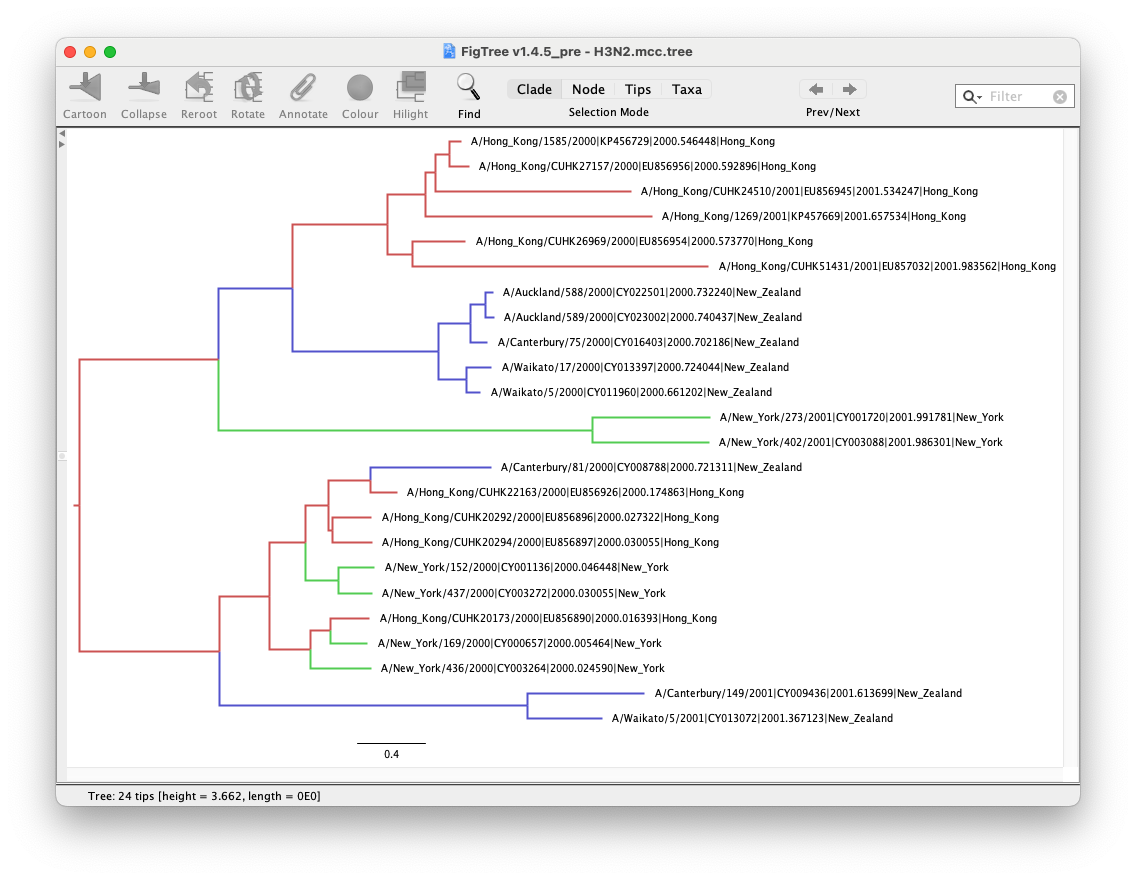
\includegraphics[width=1.000000\textwidth]{figures/figtree.mcc.png}
    \caption{MCC tree, inferred node locations.}
    \label{fig:mcc_tree}
\end{figure}

\begin{figure}
	\centering
	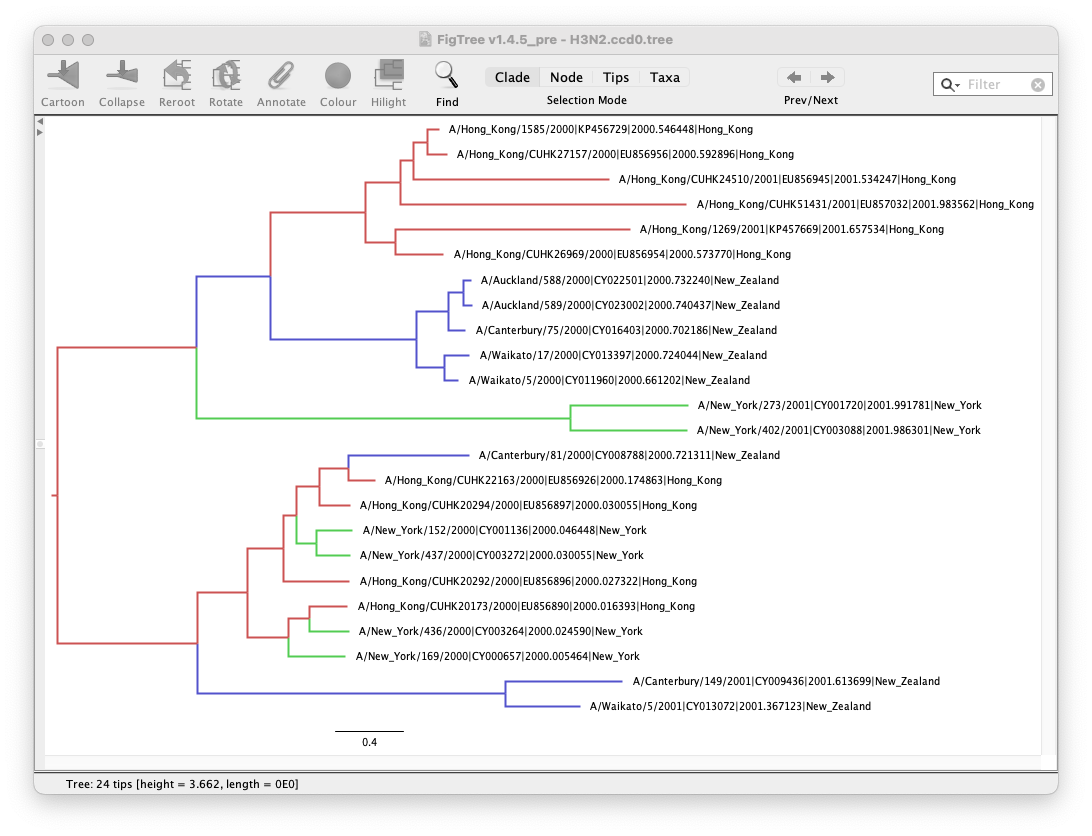
\includegraphics[width=1.000000\textwidth]{figures/figtree.ccd0.png}
	\caption{CCD0 tree, inferred node locations.}
	\label{fig:ccd0_tree}
\end{figure}

We can now determine if lineages ancestral to samples from New York are actually inferred to be from Hong Kong, or the probability of the root being in any of the locations.

To get the actual inferred probabilities of each node being in any of the 3 locations, you can go to \emph{Node Labels} \textgreater{}\textgreater{}  \emph{Display} an then choose Hong\_Kong, New\_York or New\_Zealand. These are the actual inferred probabilities of the nodes being in any location.

It should however be mentioned that the inference of nodes being in a particular location makes some simplifying assumptions, such as that there are no other locations (i.e. apart from the sampled locations) where lineages could have been.

Another important thing to know is that currently, we assume rates to be constant. This means that we assume that the population size of the different locations does not change over time. We also make the same assumption about the migration rates through time.


Now, compare the figures for MCC and CCD0 summary trees. 
\begin{framed}
	One of the CCD0 summary method advantages is that it can evaluate tree topologies that were not sampled during the MCMC. This is why it usually performs better on high-entropy (uncertain, spread out) tree posterior. Knowing this, what observations can you make about our sample? Can you see some differences?
\end{framed}

\subsubsection{Errors that can occur (Work in progress)}\label{errors-that-can-occur}

One of the errors message that can occur regularly is the following:
\emph{too many iterations, return negative infinity}.
This occurs when the integration step size of the ODE's to compute the probability of observing a phylogenetic tree in MASCOT is becoming too small.
This generally occurs if at least one migration rate is really large or at least one effective population size is really small (i.e. the coalescent rate is really high). This causes integration steps to be extremely small, which in turn would require a lot of time to compute the probability of a phylogenetic tree under MASCOT. Instead of doing that, this state is rejected by assigning its log probability the value negative infinity.

This error can have different origins and a likely incomplete list is the following:
\begin{enumerate}
\item The priors on migration rates put too much weight on really high rates. To fix this, reconsider your priors on the migration rates. Particularly, check if the prior on the migration rates make sense in comparison to the height of the tree. If, for example, the tree has a height of 1000 years, but the prior on the migration rate is exponential with mean 1, then the prior assumption is that between any two states, we expected approximately
 1000 migration events.
\item  The prior on the effective population sizes is too low, meaning that the prior on the coalescent rates (1 over the effective population size) is too high. This can for example occur when the prior on the effective population size was chosen to be 1/X. To fix, reconsider your prior on the effective population size.
\item  There is substantial changes of the effective population sizes and/or migration rates over time that are not modeled. In that case, changes in the effective population sizes or migration rates have to be explained by population structure, which can again lead to some effective population sizes being very low and some migration rates being very high. In that case, there is unfortunately not much that can be done, since MASCOT is not an appropriate model for the dataset.
\item  There is strong subpopulation structure within the different subpopulations used. In that case, reconsider if the individual sub-populations used are reasonable.
\end{enumerate}


\section{Useful Links}\label{useful-links}

If you interested in the derivations of the marginal approximation of the structured coalescent, you can find them here \citep{Mueller2017}. This paper also explains the mathematical differences to other methods such as the theory underlying BASTA. To get a better idea of how the states of internal nodes are calculated, have a look in this paper \citep{mueller2017mascot}.

\begin{itemize}

\item
  MASCOT source code: \url{https://github.com/nicfel/Mascot}
\item
  \href{http://www.beast2.org/book.html}{Bayesian Evolutionary Analysis
  with BEAST 2} \citep{BEAST2book2014}
\item
  BEAST 2 website and documentation: \url{http://www.beast2.org/}
\item
  Join the BEAST user discussion:
  \url{http://groups.google.com/group/beast-users} 
\end{itemize}





%%%%%%%%%%%%%%%%%%%%%%%
% Tutorial disclaimer %
%%%%%%%%%%%%%%%%%%%%%%%
% Please do not change the license
% Add the author names and relevant links
% Add any other aknowledgments here
\href{http://creativecommons.org/licenses/by/4.0/}{\includegraphics[scale=0.8]{figures/ccby.pdf}} This tutorial was written by Nicola F. Müller for \href{https://taming-the-beast.github.io}{Taming the BEAST} and is licensed under a \href{http://creativecommons.org/licenses/by/4.0/}{Creative Commons Attribution 4.0 International License}. 


%%%%%%%%%%%%%%%%%%%%
% Do NOT edit this %
%%%%%%%%%%%%%%%%%%%%
Version dated: \today




%%%%%%%%%%%%%%%%
%  REFERENCES  %
%%%%%%%%%%%%%%%%

\printbibliography[heading=relevref]


\end{document}